% Chapter Template

\chapter{Modeling Quran Phonetic Script} % Main chapter title

\label{Chapter5} % Change X to a consecutive number; for referencing this chapter elsewhere, use \ref{ChapterX}

\lhead{Chapter 5. \emph{Modeling Quran Phonetic Script}} % Change X to a consecutive number; this is for the header on each page - perhaps a shortened title




\section{Modeling}

Our Quran Phonetic Script produces two types of outputs: `phonemes` and `sifat` (which comprises 10 distinct attributes). We model this task as follows: Imagine processing an input speech utterance and simultaneously generating transcripts in multiple languages, such as Arabic, English, French, and German. Similarly, we implement a speech encoder with a separate linear output layer for each of our 11 levels (one for `phonemes` and 10 for the `sifat` attributes), resulting in 11 parallel transcription heads. We employ the Connectionist Temporal Classification (CTC) loss \cite{graves2006ctc} without a language model, as our objective is to transcribe the actual pronunciation rather than the intended utterance. We refer to this architecture as \textbf{Multi-level CTC}.

The total loss is computed as a weighted average of the CTC losses across all 11 levels. The `phonemes` level is assigned a weight of 0.4 due to its larger vocabulary size (43 symbols), while the remaining levels are weighted proportionally lower:

\begin{equation}
\text{loss} = \sum_{i} \left( \text{level\_weight}_i \cdot \text{CTC\_level}_i \right)
\label{eq:multilevel_ctc}
\end{equation}

We used a weight of 0.4 for the `phonemes` level, 0.0605 for both `shidda_or_rakhawa` and `tafkheem_or_taqeeq`, and 0.059875 for each of the remaining levels.

\begin{figure}[H]
\centering
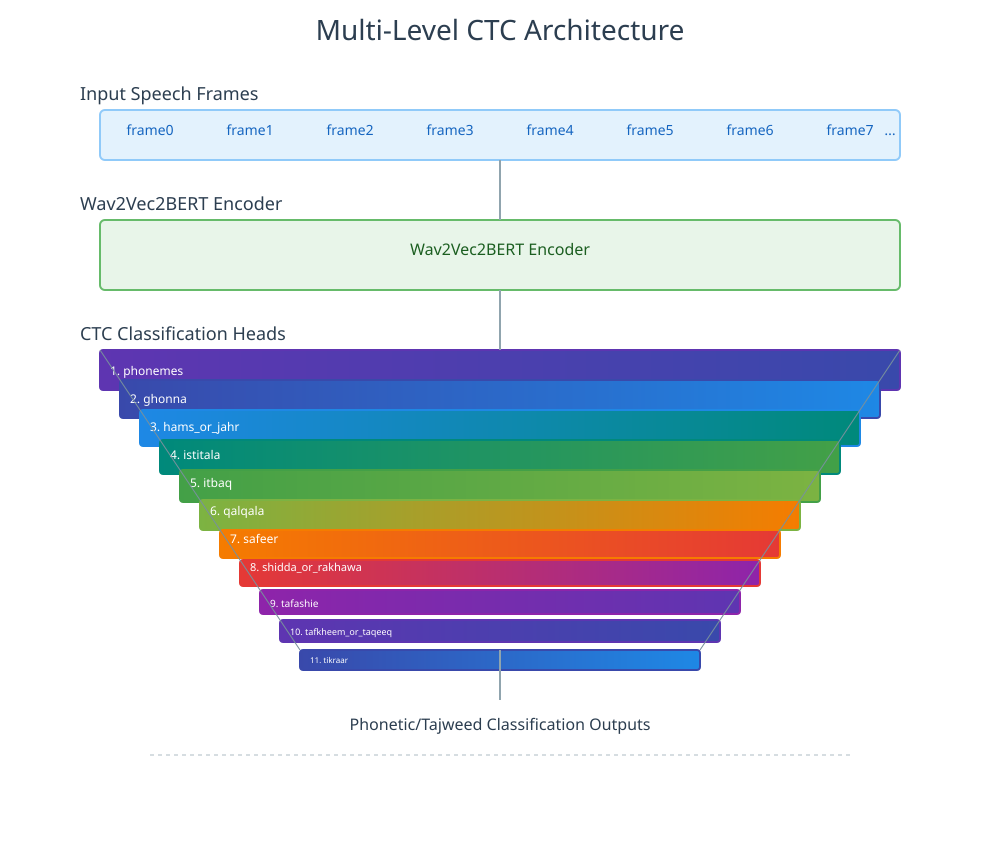
\includegraphics[width=0.8\textwidth]{../figures/multi-level-ctc.png}
\caption{Multi-level CTC architecture with 11 output heads, each computing a CTC loss, combined via weighted average.}
\label{fig:multi_level_ctc}
\end{figure}

We fine-tuned Facebook's Wav2Vec2-Bert model \cite{barrault2023seamless} for a single epoch using a constant learning rate of \texttt{5e-5}. Data augmentations were applied using the \texttt{audiomentations} library \cite{Audiomentations}, mirroring the augmentations used in Silero VAD \cite{SileroVAD}, with additional augmentations including \texttt{TimeStretch} and \texttt{GainTransition}. Samples longer than 30 seconds were filtered out to optimize GPU memory utilization—this resulted in the exclusion of only 3k samples from the 250k training set.

\begin{figure}[H]
\centering
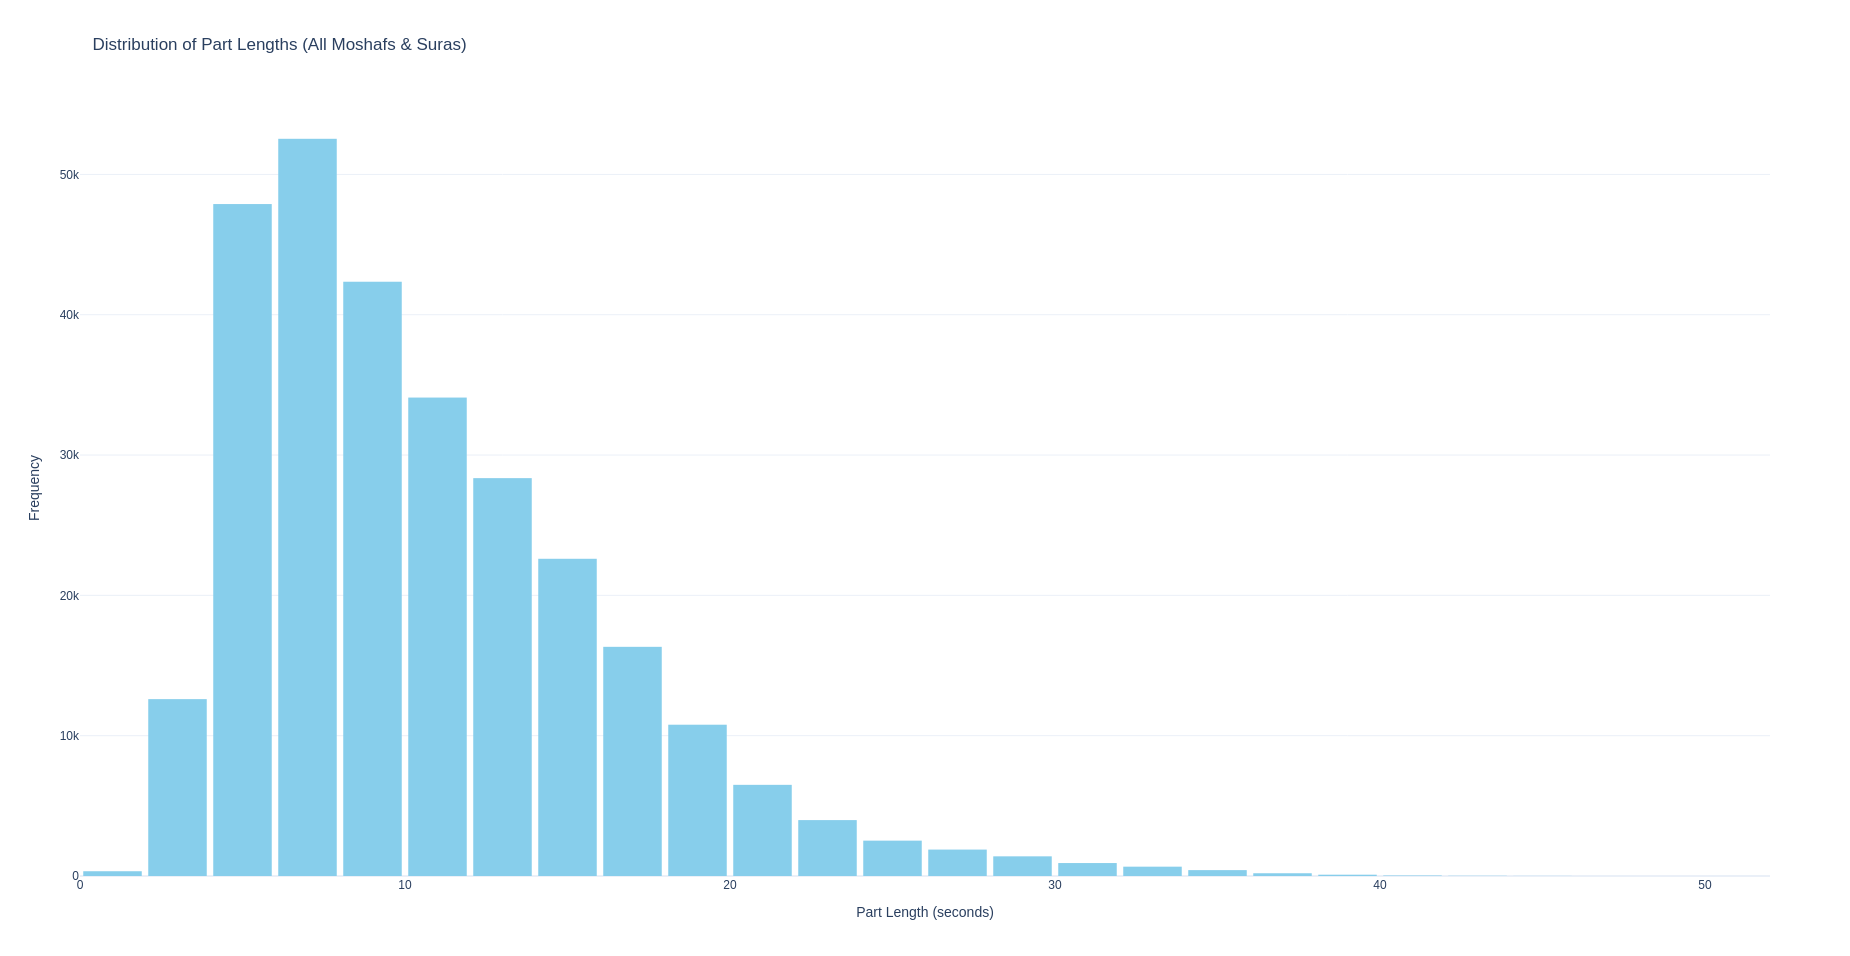
\includegraphics[width=0.8\textwidth]{./figures/audio-lens.png}
\caption{Distribution of recitation lengths (in seconds) across the dataset.}
\label{fig:audio_lens}
\end{figure}

Training was conducted on a single H200 GPU with 141 GB of memory and completed in approximately 7 hours.
